\documentclass[10pt]{article}
%\documentclass[review]{siamart1116}
%\documentclass[review]{siamonline1116}

\usepackage{amsmath}
\usepackage{amsfonts}
\usepackage{amssymb}
\usepackage{fancyhdr}
\usepackage[margin=0.75in]{geometry}
\usepackage{graphicx}
\usepackage[section]{placeins}
\usepackage{nicefrac}
\usepackage{bm}
\usepackage{xcolor}
\usepackage[format=plain,indention=.5cm, font={it,small},labelfont=bf]{caption}
\usepackage{subcaption}
\usepackage{float}
\usepackage{enumerate}
\usepackage{tikz}
\usepackage[all]{xy}
\usepackage{url}



%%%%%%%%%%%%%%%%%%%%%%%%%%%%%%%%%%%%%%%%%%%%%%%%%%%%%%%%%%%%%%%%%%%%%%%%%%%%%%%%%%%%%%%%%%%%%%%%%%%%%%%%%%%%%%%%%%
\usepackage{stackengine}
\usepackage{amsthm}
\usepackage{cleveref}


\newtheorem{theorem}{Theorem}
\newtheorem*{theorem*}{Theorem}
\newtheorem{lemma}{Lemma}
\newtheorem*{lemma*}{Lemma}
\newtheorem{conj}{Conjecture}
\newtheorem{corollary}{Corollary}
\newtheorem{clm}{Claim}
\newtheorem{rmk}{Remark}
\newtheorem{note}{NOTE}

\theoremstyle{definition}
\newtheorem*{def*}{Definition}
\newtheorem{definition}{Definition}
\numberwithin{theorem}{section}
\numberwithin{definition}{section}
\numberwithin{lemma}{section}
\numberwithin{corollary}{section}
\numberwithin{clm}{section}
\numberwithin{rmk}{section}

\newcommand{\low}[1]{$_{\text{#1}}$}
\newcommand\xput[2][0.5]{%
	\rule{#1\linewidth}{0pt}\makebox[0pt][c]{#2}\hfill}

\setlength{\headheight}{15pt}
\pagestyle{fancy}
\renewcommand{\headrulewidth}{0pt}
\fancyhead[L]{Brunner}
\fancyhead[C]{Co-Occurrance Network}
\fancyhead[R]{\today}
\lfoot{}
\cfoot{\thepage}
\rfoot{}

%%%%%%%%%%%%%%%%%%%%%%%%%%%%%%%%%%%%%%%%%%%%%%%%%%%%%%%%%%%%%%%%%%%%%%%%%%%%%%%%%%%%%%%%%%%%%%%%%%%%%%%%%%%%%%%%%%
%
%
%\newsiamthm{clm}{Claim}
%\newsiamremark{rmk}{Remark}
%\newsiamremark{note}{NOTE}
%\numberwithin{theorem}{section}
%
%
%%%%%%%%%%%%%%%%%%%%%%%%%%%%%%%%%%%%%%%%%%%%%%%%%%%%%%%%%%%%%%%%%%%%%%%%%%%%%%%%%%%%%%%%%%%%%%%%%%%%%%%%%%%%%%%%%%
\newenvironment{inbox}[1]
{\begin{center}
		\begin{tabular}{|p{0.9\textwidth}|}
			\hline\\
			{\bf #1}\\
		}
		{ 
			\\\\\hline
		\end{tabular} 
	\end{center}
}

\newcommand{\nhalf}{\nicefrac{1}{2}}
\newcommand{\eps}{\epsilon_{machine}}
\newcommand{\ol}{\overline}
\renewcommand{\b}{\bm}

\definecolor{dgreen}{RGB}{49,128,23}
\definecolor{nicepink}{RGB}{255, 0, 102}
\definecolor{nicered}{RGB}{255, 80, 80}

\newcommand{\bE}{\mathbb{E}}
\newcommand{\bP}{\mathbb{P}}
\newcommand{\bR}{\mathbb{R}}
\newcommand{\bN}{\mathbb{N}}
\newcommand{\bZ}{\mathbb{Z}}
\newcommand{\bQ}{\mathbb{Q}}
\newcommand{\bC}{\mathbb{C}}
\newcommand{\cA}{\mathcal{A}}
\newcommand{\cB}{\mathcal{B}}
\newcommand{\cC}{\mathcal{C}}
\newcommand{\cD}{\mathcal{D}}
\newcommand{\cE}{\mathcal{E}}
\newcommand{\cF}{\mathcal{F}}
\newcommand{\cG}{\mathcal{G}}
\newcommand{\cH}{\mathcal{H}}
\newcommand{\cI}{\mathcal{I}}
\newcommand{\cJ}{\mathcal{J}}
\newcommand{\cK}{\mathcal{K}}
\newcommand{\cL}{\mathcal{L}}
\newcommand{\cM}{\mathcal{M}}
\newcommand{\cN}{\mathcal{N}}
\newcommand{\cO}{\mathcal{O}}
\newcommand{\cP}{\mathcal{P}}
\newcommand{\cQ}{\mathcal{Q}}
\newcommand{\cR}{\mathcal{R}}
\newcommand{\cS}{\mathcal{S}}
\newcommand{\cT}{\mathcal{T}}
\newcommand{\cU}{\mathcal{U}}
\newcommand{\cV}{\mathcal{V}}
\newcommand{\cW}{\mathcal{W}}
\newcommand{\cX}{\mathcal{X}}
\newcommand{\cY}{\mathcal{Y}}
\newcommand{\cZ}{\mathcal{Z}}

\newcommand{\inter}{\text{\normalfont int}}
\newcommand{\ka}{\kappa}
\newcommand{\fp}{\varrho}
\newcommand{\problem}[2]{ \ \\ {\bf #1} {\it #2} \ \\} 

\renewcommand{\arraystretch}{1.5}
\renewcommand{\thefootnote}{\fnsymbol{footnote}}	
\author{Jim Brunner}
\title{Using a co-occurrance network}

\begin{document}
\maketitle
\section{Network Building}
We are looking at creating ecological networks of a microbiome. Right now, I have built two networks, in the form of graphs $\cG_1 = (\cV_1, \cE_1)$ and $\cG_2 = (\cV_2,\cE_2)$. In both graphs, vertex are labeled by taxa name. I'm going to conflate the vertices and their label. The edge sets are defined by co-incidence and co-occurence, respectively. Given a set of samples with abundancs of organisms, we map the abundances to discrete levels, as proportions of the maximum abundance \emph{of that organism}. Precisely, let the samples be $s_i$ and raw abundance of organism $j$ in sample $i$ be $r_{ji}$. I map the abundances according to
\[
a(r_{ji})  = \left\{
\begin{array}{c c}
\lfloor\left(\frac{r_{ji}}{\max_{s_k}(r_{jk})}\right) n \rfloor + 1 &  \frac{r_{ji}}{\max_{s_k}(r_{jk})} \geq m \\
0 & \frac{r_{ji}}{\max_{s_k}(r_{jk})} < m
\end{array}
\right.
\]
where $m$ is some minimum. Then, I create weighted edges between vertices (where $0$ weight means no edge exists) where the weights of edges in $\cE_1$ are
\[
w^1_{jk} = \frac{\|\{i: a(r_{ji}) = a(r_{ki}) \neq 0\} \|}{S}
\]
where $S$ is the total number of samples. That is, we count the propotion of samples in which the two taxa appear at the same discritized level. 

The second network accounts for random coincidence of taxa in a sample, following \cite{coocc}. It begins with $\cG_1$, and compares to a null model $N$. The null model is defined in the following way.
\[
A_j= \sum_{s_i} \b{1}_{a(r_{ji}) \neq 0}
\] 
and 
\[
S_i^l  = \sum_{v_j} \b{1}_{a(r_{ji}) = l}
\]
Then, $N$ assumes that if
\[
X_{jil} \sim \mathit{binom}\left(A_j, \frac{S_i^l}{\sum_{il} S_i^l}\right)
\]
then $P(a_{ji}^N = l) = 1-P(X_{jil} = 0)$. This allows us to calculate the probability of co-incidence of taxa under the null model. Let $w_{jk}^N$ be
\[
w^N_{jk} = \|\{i: a_{ji}^N = a_{ki}^N \neq 0\} \|
\]
This is the similar to the co-incidence model but now randomized. Then,
\[
P(w_{jk}^N = K) =  \sum_{\{A \subset \cV_2:|A| = k\}} \prod_{l\in A} a_{jl}a_{kl}\prod_{l \not\in A} (1- a_{jl}a_{kl})
\]
Ideally, we would then define $\cE_2$ by the weights
\[
w_{jk}^2 = \left\{ \begin{array}{c c}
1 & P(w_{jk}^N \geq w_{jk}^1) \leq t\\
0 & P(w_{jk}^N < w_{jk}^1) > t
\end{array}\right.
\]
However, that probability is intractible to compute. Instead, we take 
\[
\widetilde{P}(w_{jk}^N = K) = \sum_{l=0}^i \binom{N_1}{l}\binom{N_2}{K-l} p_1^j p_2^{K-l} (1-p_1)^{N-l}(1-p_2)^{N-K+l}
\]
where
\[
p_1 = p_a - \left(\frac{N_2}{N_1}\frac{N(\mu-\sigma^2)- \mu^2}{N^2}\right)^{\nhalf}
\]
and 
\[
p_2 = p_a - \left(\frac{N_1}{N_2}\frac{N(\mu-\sigma^2)- \mu^2}{N^2}\right)^{\nhalf}
\]
Finally, $N_1$, $N_2$ are to ensure that $p_1,p_2 \in [0,1]$. It turns out we need:
\[
\frac{\mu N (1-p_a) - N\sigma^2}{N(1-p_a)- \sigma^2} \leq N_2 \leq \frac{\mu^2}{\mu- \sigma^2}
\]
with $\mu$ the mean of the real distrubution, $\sigma^2$ the variance, and $p_a = \frac{1}{S}\sum_{i} a_{ji}a_{ki}$. So, we take 
\[
w_{jk}^2 = \left\{ \begin{array}{c c}
1 & \widetilde{P}(w_{jk}^N \geq w_{jk}^1) \geq t\\
0 & \widetilde{P}(w_{jk}^N < w_{jk}^1) > t
\end{array}\right.
\]

\subsection{An alternative coincidence construction}
A faster way would be to first normalize abundance vectors, and just take 
\[
W = AA^T
\]
(with the diagonal reset to 0) to be the weighted adjacency matrix, where $A$ is the matrix of abundances. Then, each entry is the cosine of the angle between the abundance vectors. This also allows us to look at negatively aligned abundance vectors.

How then would we construct the cooccurrence network? Basically, what would our null model be? Well, we would still randomize the sample data. That is, we could take $X_{ij}$ be a random variable representing the abundance of taxa $i$ in sample $j$, and require that $\|X_{i}\| = 1$. Then, we can ask $P(\b{X}_i \cdot \b{X}_k > w_{ik})$. I just don't know what distribution to put on the $X_{ij}$ (the random abundances). I'll start with a binomial:
\[
P(\tilde{X}_{ij} = k) = \binom{n}{k}p^1(1-p)^{n-k}
\]
where $p = \frac{\mathit{deg}(s_j)}{\sum_l \mathit{deg}(s_l)}$ and $n =\lfloor \frac{1}{\min_{k}(r_{ik})}r_i\rfloor$ where $r_i = \sum_k r_{ik}$. Then I normalize to the unit sphere.  Finally, I can use a Monte-Carlo simulation to see which weights to check. To do this, I generate random matrices with the appropriate distributions, using a built in Numpy method. Then I check the proportion of random entries larger than the weights. If this is small, I keep the edge. Unfortunately, I can't use a control variate or otherwise try to reduce variance, because generating my own samples was far slower than the Numpy method. The Numpy method is pre-compiled in C. Variance was $\sim 0.25$, so $1000$ samples should be enough. 

Similary to the above but maybe on more established footing is Pearson's correlation coefficient. That is:
\[
\rho_{xy} = \frac{1}{N}\frac{(\b{x}- \mu_x\b{1}) \cdot (\b{y} - \mu_y\b{1})}{\sigma_x \sigma_y}
\]
which can of course be constructed by modifying the data matrix and then multiplying with it's transpose. In expectation, this the covariance divided by the product of the variances. I can also use a Monte-Carlo approach to check significance.
This ends up keeping a lot more edges than the binning procedure. I am considering doing a first pass of only keeping hgih weights. Low weights may be significant (i.e. higher than one could expect randomly) but are still low, and so maybe should be dropped. In the literature, people tend to only keep weights over $0.8$ or something.


\section{Network Analysis}
We can cluster - community clustering, spectral clustering, comparing to random graphs. Comparison of clusters to grouping by sample type.

Community clustering minimizes a funciton of the graph called modularity \cite{PhysRevE.70.066111}\cite{PhysRevE.70.056131}. That is 
\[
Q = \frac{1}{2m}\sum_{i,j}\left(w_{ij} + \frac{d_id_j}{2m}\right) \delta(c_i,c_j)
\]
where $m = \sum_{i\sim j} w_{ij}$, $d_i$ is the (weighted) degree of vertex $i$, $c_i$ is the community containing vertex $i$, and $\delta$ is the Kronecker $\delta$. This done by a kind of gradient search/greedy algorithm.

Spectral clustering performs a $k$-means clustering on the rows of the matrix whose columns are the $k$ eigenvectors of the graph laplacian corresponding to the smallest $k$ eigenvalues \cite{vonLuxburg2007} . Morally, this means it clusters points together that are close in the first $k$ (slowest decaying!) modes of the diffusion equation on the graph.
\section{Using the network to analyze a sample}

The question now is what can we do these networks?

First, assesing GOTTCHA reads. A single GOTTCHA read would produce a network with each connected component complete. I think the co-incidence network is more appropriate. We want to assess the probability that you see this set together. We have the probability that you see any vertex pair (estimated) as the edge weights of $\cG_1$. Precisely, the edge weights are
\[
w^1_{jk} = P(j \, \&\, k \in  S_i^l)
\]
where $S_i^l$ is sample $i$ at discrete abundance level $l$. It might be useful to have the directed weight graph where
\[
w^3_{jk} = P(j \in S_i^l | k \in S_i^l)
\]
but that wouldn't be hard, because then
\[
w^3_{jk} = S\frac{w^1_{jk}}{\|\{i:a(r_{ki})>0\}\|} 
\]
Anyway, let's start with the simplest case of one abundance level. Assume GOTTCHA found taxa $a,b,c,...,n$. Maybe the first thing we would want is
\[
P(a | b,c,d,...,n), \, P(b|a,c,d,...,n) ,\, \mathit{etc}
\]
Clearly, we can see directly $P(a|b)$, etc. We can also get a bound for triplets (assuming $P(c,b) \neq 0$):
\[
P(a|b,c) \leq \frac{\min_{(i,j) \subset \{a,b,c\}}(P(i,j))}{P(b,c)}
\]
but we can't do any better than triplets explicitly, because we don't have any sort of independence (conditional or otherwise) and because our network is not acyclic. 

We can probably learn something from asking about the connectivity of the induced subgraph. Notice that if it isn't complete, then one of the $P(a,b)$ is $0$ above. 

What does the connectivity of the induced subgraph of $\cG_2$ tell us? If it is connected, that's good.  We could use that network to identify vertices that are connected to many of the vertices in the induced subgraph - this might indicate that node should be in the sample.

I guess $\cG_2$ is a markov random field \cite{machine_learning}. This might give us a way to calculate the probability you see a group taxa (and maybe others). The main idea of a MRF is that nodes are conditionally independent of nodes they aren't neighbors of (conditioned on ones they are neighbors of). If $c$ are the (maximal) cliques of the graph (complete subgraphs), then the probability of configuration $\b{x}$ is
\[
P(\b{x}) = \frac{1}{Z} \prod_{c} \psi_c (x_{c})
\]	
where $Z$ is a normalizing constant and $\psi_c$ are potential functions I don't know how to come up with yet. Anyway, if we have a sample that contains (maybe as a subset) $s$, we can calculate something. Let $C_s$ be the cliques represented in $s$.
\[
P(\b{s}) = \frac{1}{Z}\sum_{\{\b{x} : s\subset \b{x}\}}\prod_{c\in C_s}\psi_c(\b{x})
\]
And we can ignore cliques not represented in $s$. We probably have to change $Z$. I guess we can also use neighbor pairs instead of maximal cliques. Either way we have to figure out what $\psi_c$ are.

\subsection{Determining $\psi_c$}

Before figuring out $\psi_c$, it should be noted that we have a choice of configuration space of the network. We can use a binary $\{1,0\}^N$ space to denote presence or absence, or we can choose a continuous space to include abundances. To begin, I will only consider presence \& absence.
	
\begin{inbox}{Snowshoe hairs and Canadian Lynx, CRNT}
Now I'm very tempted to think about how this approach relates to mass action dynamical systems. I'm going to think about my very favorite model.
\[
\b{\dot{x}} = \ka_1 x \begin{pmatrix} 1 \\ 0 \end{pmatrix} + \ka_2 xy \begin{pmatrix}
-1 \\ 1
\end{pmatrix} + \ka_3 y \begin{pmatrix}
0\\-1
\end{pmatrix}
\]
Well. Yes. But there is only one maximal clique so $P(\b{x}) = \psi (\b{x})$ and that's just whatever it is. We know that it evolves according to the stochastic mass action equations. In fact, the result that the stationary distribution is a product of poissons for a complex balanced system can be thought of as fitting into this framework. I wonder if you could use this theory to re-prove that? Recall that the stationary distribution for a complex balanced system with equilibrium $\b{c}$ is 
\[
\pi(\b{x}) = \frac{1}{Z} \prod_{i=1}^d \frac{c_i^{x_i}}{x_i!}
\]
so here we have that
\[
\psi_c = \prod_{i \in c} \frac{c_i^{x_i}}{x_i!}
\]
or taking cliques to be just singletons
\[
\psi_i = \frac{c_i^{x_i}}{x_i !}
\]	
I can't think of any way to arrive upon that directly, and so prove the result from this direction. Also, This is even more general than a MRF, as it has self-loops. Self loops play the role of time update. In fact, one might say that a MC is to a MRF as an ODE is to a PDE. Then, self loops in the MRF correspond to time derivatives or forcing appearing in the PDE.
\end{inbox}

It seems reasonable to use a pairwise RMF. It also seems reasonable to take a log linear function. My initial guess is
\[
\psi_{s\sim t} (y_s,y_t) = \exp(\b{\theta} \cdot \b{1}_{y_s = i,y_t = j})
\]
where $\theta = (0,\log(P(s)), \log(P(t)),\log(\nhalf(P(s|t) + P(t|s))))$. But that's a guess. It makes sense we have only unconnected nodes. It also also penalizes leaving out nodes that are connected to the nodes we do have. However, this penalizes us too harshly if we include a hub node.

Let's play with a small network to try to get a handle on this. Consider the network shown in \cref{toy_network}
\begin{figure}
	\begin{center}
	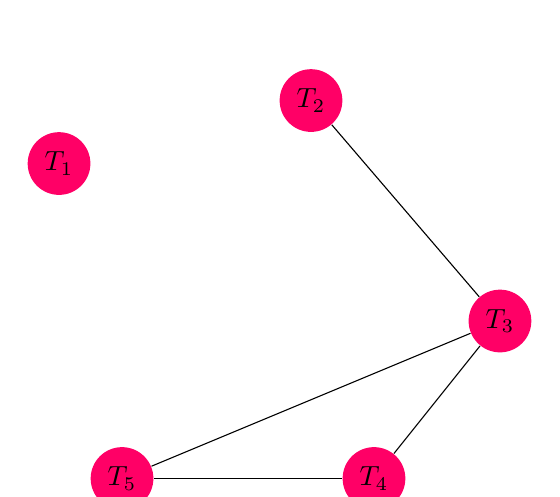
\begin{tikzpicture}[scale = 4]
	\node (a) at (0,1) [circle, fill = nicepink] {$T_1$};
	\node (b) at (0.8,1.2) [circle, fill = nicepink] {$T_2$};
	\node (c) at (1.4,0.5) [circle, fill = nicepink] {$T_3$};
	\node (d) at (1,0) [circle, fill = nicepink] {$T_4$};
	\node (e) at (0.2,0) [circle, fill = nicepink] {$T_5$};
	\draw (b) edge (c);
	\draw (c) edge (d);
	\draw (c) edge (e);
	\draw (d) edge (e);
	\end{tikzpicture}
	\end{center}
	\caption{A small network example}\label{toy_network}
\end{figure}
I think we can assume that
\[
p(\b{x}) = \prod_{s\sim t} \psi_{st}(\b{x})\prod_{s}\psi_s(\b{x})
\]
To start, we should think about the distribution of an independent node ($T_1$). Clearly
\[
P(T_1 = x) = \psi_{1}(x)
\]
Similarly, we should have
\[
P(T_2 = x) = \psi_2(x) = \int \psi_2(x)\psi_{23}(y) dy =  \bE (P(T_2 = x|T_3))   
\]
Maybe a binomial is a good idea:
\[
P\left(T_1 = \frac{k}{N}\right) = \binom{N}{k}p^k(1-p)^{N-k}
\]
where $p$ is something like the proportion of times $T_1$ appears in the data, the sum of abundances of $T_1$ in the data divided by $N$. $N$ is some scaling parameter, like the largest total abundance or something. But then, it's natural to take $N$ large and get a Gaussian by the CLT. So maybe we do a multivariate Guassian. Then
\[
\psi_{s\sim t}(\b{x}) = \exp\left(-\frac{1}{2} x_s \Lambda_{st}x_t\right)
\]
and
\[
\psi_s(\b{x}) = \exp\left(\eta_s x_s - \Lambda_{ss}x_s^2\right)
\]
\cite{machine_learning}. We already have the covariance (normalized by the product of the standard deviations) matrix $\Sigma$, in the Pearson coefficient. So, we have $\Lambda = \Sigma^{-1}$, and $\b{\eta} = \Sigma^{-1}\b{\mu}$. Unfortunately, $\Sigma$ is singular, it's dimension is bounded by the number of samples I have. This of course leaves us in the wind when it comes to $\Lambda$. So, I suppose we have to try to approximate $\Lambda$ subject to the constraint that if $s \not\sim t$, $\Lambda_{st} = 0$. We can use the SVD:
\[
\Sigma = M S N^* \Rightarrow \Sigma^+ = N \tilde{S} M^*
\] 
where $\tilde{S}$ is diagonal with $1/s_i$ until you get to zero singular values, where you just put a $0$. Because $\Sigma$ is symmetric, we have $M^* = N$. Then,
\[
\Sigma^+ = N \tilde{S} N
\]
I guess this is used, although it doesn't seem to preserve zeros. There's a function in scipy.

On the other hand, taking $N$ large and $p$ small we get an exponential random variable. So perhaps I want
\[
\psi_1(x) = e^{-\lambda}\frac{\lambda^{Nx}}{(Nx)!}
\]
or more directly
\[
\psi_1(x) = \binom{N}{Nx}p^{Nx}(1-p)^{N-Nx}
\]
and using Stirling's formula,
\[
\log(\psi_1) \approx N\left[x \log\left(\frac{p}{x}\right) + (1-x)\log\left(\frac{1-p}{1-x}\right)\right]
\]

\subsection{Comparing configurations without specifying $\psi$}
Mayby I don't need to figure out $\psi_{st}$ and $\psi_s$. Maybe I can conclude something like 
\[
\frac{P(\b{x})}{P(\b{y})} > 1
\]
without knowing them. For that, I would need to just identify which cliques change, and ask whether they increase or decrease. How exactly to decide that is a question. Probably single nodes we wouldn't change. For a clique, we could assume that $\psi_c$ decreases if we have over half the nodes and reduce and still have at least half, but increase if the we have less than half and decrease. That is, let $c$ be a clique with $n$ members, and $\psi_c(k)$ be the value of $\psi_c$ with $k$ members ``on". Then
\[
\frac{\psi_c(k+1)}{\psi_c(k)}   \left\{\begin{array}{c c}
>1 & k>\nicefrac{n}{2}\\
<1 & k\leq \nicefrac{n}{2}
\end{array}\right.
\]
Then, we are basically asserting the cliques like to either be all there or none there. Which seems good.

Here the algorithm for deciding which of two nodes should be on and which should be off would be:
\begin{enumerate}[(i)]
	\item Identify cliques $c_1,...,c_m$ which contain one or both nodes
	\item compute $\frac{\psi_{c_i}(k^1)}{\psi_{c_i}(k^2)}$ for each  $i \in \{1,...,m\}$, where $k^j$ is the number of members present in configuration $j \in \{1,2\}$, and this fraction is computed according to a simple rule of the kind above.
	\item multiply these ratios: $\frac{P(\text{configuration 1})}{P(\text{configuration 2})} = \prod_{i=1}^k \frac{\psi_{c_i}(k^1)}{\psi_{c_i}(k^2)}$
\end{enumerate}

I need to specify that rule. The simplest reasonable thing is probably linear
\[
\frac{\psi_c(k+1)}{\psi_c(k)} = \frac{2(1-r_{min})}{n - 1} k + r_{min}
\]
but one could imagine some kind of sigmoidal rule as well, so that around $\nicefrac{n}{2}$ this ratio is close to $1$. This makes sense on a $2$ clique, as it implies that
\[
\psi(2) > \psi(1) \; \& \; \psi(0) > \psi(1)
\]
and in general makes sense for $n$ even. It makes sense for $n$ odd as well. It asserts that it is equally likely to have on $\nicefrac{n}{2} \pm \nicefrac{1}{2}$. Finally, if we need to compare $k$ and $k+2$, we simply take
\[
\frac{\psi(k+2)}{\psi(k)} = \frac{\psi(k+2)}{\psi(k+1)}\frac{\psi(k+1)}{\psi(k)}
\]
That is, a discrete analogue to the chain rule.
\subsection{Diffusion based method.}
Here's an idea inspired by spectral clustering: Solve the diffusion equation on the graph:
\[
\frac{\partial}{\partial t} u(v,t) = L u(v,t)
\]
where $v$ takes values in the vertex set of the graph. Put the initial mass on nodes you are confident in or something like that. Then, compare
\[
U(v) = \int_{0}^{\infty} u(v,t) dt
\]
Higher should be more likely. This should tell us something like $P(v|v_{initial})$. I'll need to prove that. Let's go ahead and formulate the conjecture.

\begin{conj}\label{initalCond}
Consider a random markov field with configurations in $\{0,1\}^N$. Assume that $P(v_i = 1|v_j = 1) \geq P(v_i = 1)$, with strict inequality if and only if there exists an edge connecting $v_i$ and $v_j$. Consider two configurations $\b{x}$ and $\b{y}$ which differ only in two nodes, so that in $\b{x}$ we have $\b{x}(v_1) = 1$, $\b{x}(v_2) = 0$ and in the other $\b{y}(v_1) = 0$ and $\b{y}(v_2) = 1$.

Let $u_i(t)$ be the solution at node $v_i$ to the discete diffusion problem
\[
\frac{d}{dt}\b{u}(t)  = - L\b{u}
\]
where $L$ is the  graph laplacian with initial conditions $u_1 = u_2 = 0$ and other nodes initialized to $0$ or $1$ according $\b{x}$ and $\b{y}$, and no-flux boundary conditions. 

Then, 
\[
\int_0^{\infty} u_1(t) dt > \int_0^{\infty} u_2(t) dt  \Leftrightarrow  P(\b{x}) > P(\b{y})
\]
\end{conj}

or alternatively...

\begin{conj}\label{boundarVal}
	Consider a random markov field with configurations in $\{0,1\}^N$. Assume that $P(v_i = 1|v_j = 1) \geq P(v_i = 1)$, with strict inequality if and only if there exists an edge connecting $v_i$ and $v_j$. Suppose that $m$ node values are known. Let $u_i(t)$ be the the solution to
	\[
	\frac{d}{dt}\b{u}(t) = -L\b{u}
	\]
	where $L$ is the graph Laplacian, we have initial conditions $0$ for unknown nodes and known node vales fixed (as a boundary condition). Then,
	\[
	\lim_{t\rightarrow \infty} u_i(t) >\lim_{t\rightarrow \infty} u_j(t) \Leftrightarrow P(v_i = 1|\text{ known node values}) > P(v_j = 1 | \text{ known node values})
	\]
\end{conj}

We really just need the $\Rightarrow$ direction. It would also be nice to expand to a set of unknown nodes. The natural extension is to specify a known subset and ranking unknown nodes based on the above.

\begin{proof}[proof (\cref{initalCond}).]
	($\int_0^{\infty} u_1(t) dt > \int_0^{\infty} u_2(t) dt  \Rightarrow  P(\b{x}) > P(\b{y})$). We can show this by showing that 
	\[
	\prod_{\{c|v_1 \in c \,\mathit{or}\, v_2 \in c\}}\frac{\psi_c(\b{x})}{\psi_c(\b{y})} >1
	\]
\end{proof}

\begin{proof}[proof (\cref{boundarVal}).]
	We hope to prove this by constructing a dynamical system with the desired property, because it is likely this will be the diffusion equation on the graph. Or maybe not. I don't know....
	
	Consider a Baysian network. Seems like it works there.
\end{proof}
	
\bibliographystyle{plain}
\bibliography{../../summer17}
\end{document}